%UNIT 9: INTRODUCTION TO SYSTEMS
%%%%%%%%%%%%%%%%%%%%%%%%%%%
%%%% Put the following at the top of each .tex file  %
\pagestyle{fancy}
\renewcommand{\theUnit}{5.4}
\ifthenelse{\isundefined{\UnitPageNumbers}}{}{\setcounter{page}{1}}
\rhead{Section \theUnit: Introduction to Systems}
\lhead{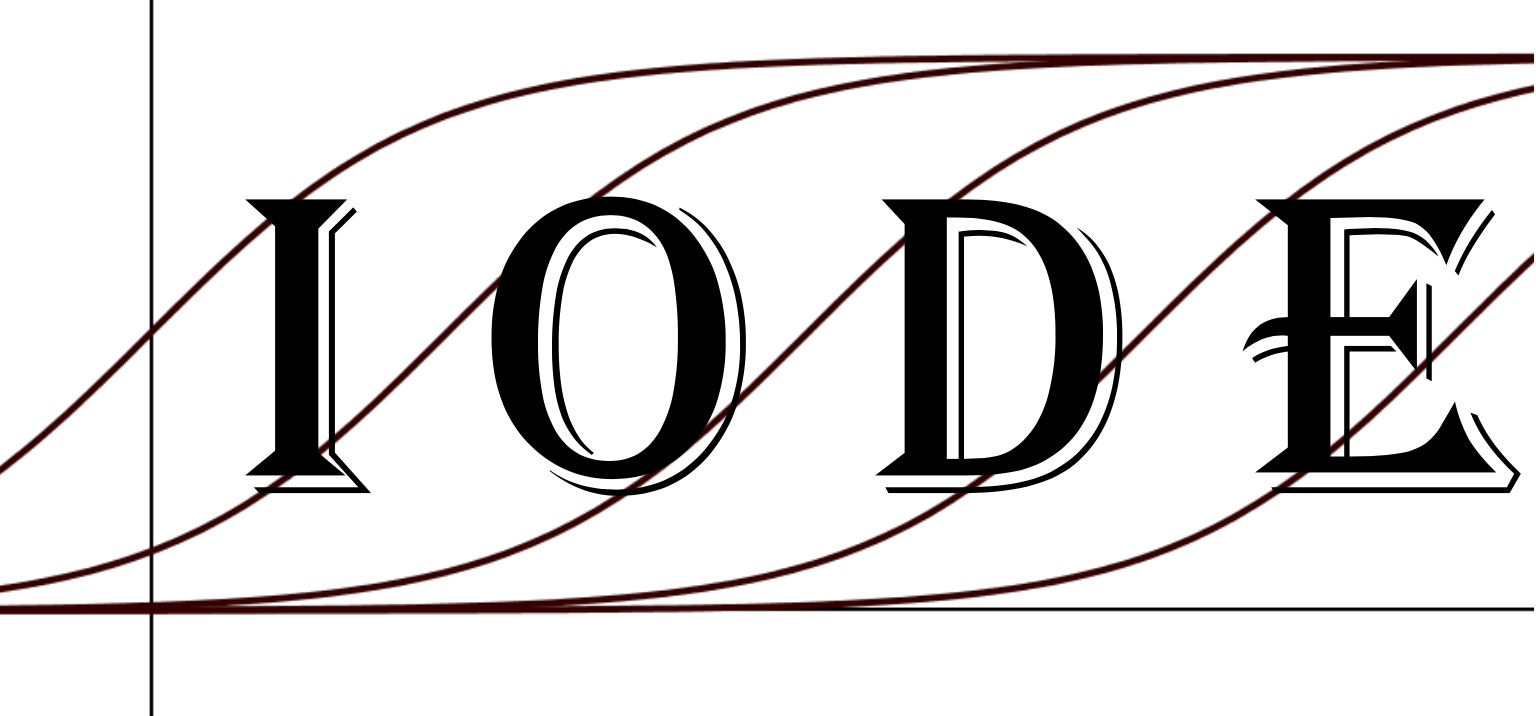
\includegraphics[width=1.25cm]{IODE-logo.png}}
\rfoot{\mypage}
\lfoot{}
\cfoot{}
\fancypagestyle{firstfooter}{\footskip = 50pt}
\renewcommand{\footrulewidth}{.4pt}
%%%%%%%%%%%%%%%%%%%%%%%%%%%
\vspace*{-20pt} \thispagestyle{firstfooter}
\pagebegin{Rabbits and Foxes}

Most species live in interaction with other species. For example, perhaps one species preys on another species, like foxes and rabbits. Below is a \textbf{system of rate of change equations} intended to predict future populations of rabbits and foxes over time, where $R$ is the population (in hundreds) of rabbits at any time $t$ and $F$ is the population of foxes (in tens) at any time $t$ (in years).
 \begin{align*}
	\frac{dR}{dt} &= 3R-1.4RF\\
	\frac{dF}{dt} &= -F+0.8RF
 \end{align*}

\begin{enumerate}
\item \label{09problem1}
\begin{enumerate}
\item In earlier work with the rate of change equation $\frac{dP}{dt}=kP$  we assumed that there was only one species, that the resources were unlimited, and that the species reproduced continuously. Which, if any, of these assumptions is modified and how is this modification reflected in the above system of differential equations? \label{09problem1parta} \vfill

\item   Interpret the meaning of \emph{each} term in the rate of change equations (e.g., how do you interpret or make sense of the $-1.4RF$ term) and what are the implications of this term on the future predicted populations? Similarly for $3R$, $-F$, and $0.8RF$. \label{09problem1partb}
\vfill

\end{enumerate}
\item \label{09problem2}
Scientists studying a rabbit-fox population estimate that the current number of rabbits is 100 ($R=1$) and that the number of foxes is 10 ($F=1$). Use two steps of Euler's method with step size of $\Delta t =0.5$ to get numerical estimates for the future number of rabbits and foxes as predicted by the differential equations. \label{09problem2parta}

\begin{tabular}{|c|c|c|c|c|c|c|}
\hline
 $t$	& $R$ (in hundreds)	& $F$ (in tens) & $\dsty \frac{dR}{dt}$ & $\Delta R$ & $\dsty \frac{dF}{dt}$ & $\Delta F$ \\
 \hline
 & & & \ \ \ \ \ \ \ \ \ \ \ \ \ \ \ \ \ \ \ \ &  \ \ \ \ \ \ \ \ \ \ \ \ \ \ \ \ \ \ \ \  &  \ \ \ \ \ \ \ \ \ \ \ \ \ \ \ \ \ \ \ \  &  \ \ \ \ \ \ \ \ \ \ \ \ \ \ \ \ \ \ \ \ \\ 
0 & 1 & 1& & & & \\
&  & & & & & \\
\hline
&  & & & & & \\
0.5 & & & & & & \\
&  & & & & & \\
\hline
&  & & & & & \\
1.0 & & & & & &\\
&  & & & & & \\
\hline		
\end{tabular}
\vfill

%\item	What are some different two dimensional and three dimensional ways to graphically depict your $(t, R, F)$ values? \label{09problem2partb}

\vfill
%\end{enumerate}
%\end{enumerate}
\clearpage

%%%%%%%%%%%%%%%%%%%%%%%%%
%\pagebegin{Three Dimensional Visualization} 
%\begin{enumerate}[resume]
%\item 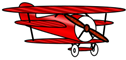
\includegraphics{11/11fig1} A crop duster plane with a two blade propeller is rolling along a runway. On the end of one of the propeller blades, which are rotating clockwise at a slow constant speed, is a noticeable red paint mark. Imagine that for the first several rotations of the propeller blades the red mark leaves a ``trace'' in the air as the plane makes its way down the runway.  \label{09problem3}

%\begin{enumerate}
%\item Simulate this scenario over time with a pipe cleaner. On appropriate combinations of the $x$, $y$, and $t$ axes, sketch what Angler, Sider, Fronter, and Topper would ideally see assuming that they could always see the red mark. What view do you think is best and why? \label{09problem3parta}

%\begin{tikzpicture}
%\node at (4,6) {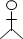
\includegraphics[]{11/11fig2}};
%\node at (7.5,6.5) {\textbf{Topper} is directly above};
%\node at (7.5,6) {the runway in a hot air balloon};
%\node at (7.5,5.5) {moving with the airplane};
%\node at (5,4) {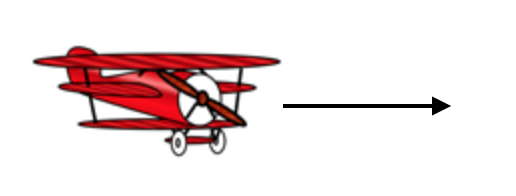
\includegraphics[width=2in]{11/11fig3}}; 
%\node at (12,4) {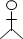
\includegraphics[]{11/11fig2}};
%\node at (11,4) {\textbf{Fronter}};
%\node at (11.5,3) {is on a truck moving};
%\node at (11.5,2.5) {at the same speed};
%\node at (11.5,2) {as the airplane};
%\node at (1,2) {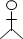
\includegraphics[]{11/11fig2}};
%\node at (0,2) {\textbf{Angler}};
%\node at (1,1) {behind and off to the};
%\node at (1,0.5) {side of the airplane};
%\node at (1,0) {moving with the airplane};
%\node at (4,0.5) {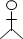
\includegraphics[]{11/11fig2}};
%\node at (7,1) {\textbf{Sider} is on the runway};
%\node at (7,0.5) {moving with the airplane};
%\node at (7,0) {from the side};
%\end{tikzpicture}

%\vfill
%Sketch your ideas for each of the following:
%\medskip

%\item	What if there was another paint mark on other end of the propeller, what, \textbf{ideally}, do the four observers see then? How does the trace of this mark relate to the previous trace?\label{09problem3partb}\vfill
%\item	What if there was a paint mark on the center of the propeller blade mechanism. What do the observers ideally see then?\label{09problem3partc}\vfill
%\item	How ideally would each observer see all of the above paint marks simultaneously?\label{09problem3partd}
%\vfill
%\end{enumerate}

%\clearpage

\item	\label{09problem4}
\begin{enumerate}
\item For the system of differential equations from problem \ref{09problem1},   
\begin{align*}
\frac{dR}{dt} &= 3R-1.4RF \\
\frac{dF}{dt} &= -F+0.8RF
\end{align*}
%consider the perspectives of Angler, Sider, Fronter, and Topper. What are the coordinate axes that correspond to each? \label{09problem4parta} \vfill
%\item
use the GeoGebra applet \href{https://ggbm.at/U3U6MsyA}{\underline{https://ggbm.at/U3U6MsyA}} to generate predictions for the future number of rabbits and foxes if at time 0 we initially have 300 rabbits ($R=3$) and 20 foxes ($F=2$). Sketch graphs of $R$ vs $t$, $F$ vs $t$, and $F$ vs $R$. \label{09problem4parta} \vfill

\vspace{-3.9in}\hspace{-0.75in}
\includegraphics[width=0.5in]{11/11DEExplorerQR.png}
\vfill
%\item Use the same GeoGebra applet from problem \ref{09problem4partb} to experiment with different initial conditions and interpret the nature of the numerical solutions in the context of Rabbits and Foxes. \label{09problem4partc} \vfill
%\item	Determine an initial rabbit and fox population at time 0 such that the 3D graph of the solution is a shift of the 3D graph in problem \ref{09problem4partb} along the $t$-axis. What connections does this problem have to do with your study of autonomous first order differential equations? \label{09problem4partd} \vfill
%\end{enumerate}
\item Using initial condition $R = 3$ (300 rabbits) and $F = 2$ (20 foxes), tell the story of what happens to the rabbit and fox population as time continues. \label{09problem4partb}
\vfill
\end{enumerate}

\clearpage
\item \label{09problem5}	\begin{enumerate}
\item Suppose the current number of rabbits is $R=3$ (300 rabbits)  and the number of foxes is 0. Without using any technology and without making any calculations, what does the system of rate of change equations (same one as problem \ref{09problem4parta}) predict for the future number of rabbits and foxes? Explain your reasoning. \label{09problem5parta}
\vfill
\item Use the same GeoGebra applet from problem \ref{09problem4partb} to generate the 3D plot and all three different views or projections of the 3D plot. Show each graph and explain how each illustrates your conclusion in problem \ref{09problem5parta}. \label{09problem5partb}
\vfill
\item Using initial condition $R = 3$ (300 rabbits) and $F = 0$ (no foxes), tell the story of what happens to the rabbit and fox population as time continues. \label{09problem5partc}
\vfill
\end{enumerate} 

\item \label{09problem6}
\begin{enumerate}
\item  What would it mean for the rabbit-fox system to be in equilibrium? Are there any equilibrium solutions to this system of rate of change equations? If so, determine all equilibrium solutions and generate the 3D and other views for each equilibrium solution. \label{09problem6parta}
\vfill

\item For single differential equations, we classified equilibrium solutions as stable (attractors), unstable repellers, and semi-stable (nodes).  For each of the equilibrium solutions in the previous problem, create your own terms to classify the equilibrium solutions in \ref{09problem6parta} and briefly explain your reasons behind your choice of terms. \label{09problem6partb}
\vfill
\end{enumerate}

%\clearpage
%\item A group of scientists wants to graphically display the predictions for many different non-negative initial conditions (this includes 0 values for $R$ and $F$, but not negative values) to the rabbit-fox system of differential equations and they want to do so using only one set of axes. What one single set of axes would you recommend that they use ($R-F-t$ axes, $t-R$ axes, $t-F$ axes, or $R-F$ axes)? Explain. \label{09problem7} \vfill

\clearpage
\item One view of solutions for studying solutions to systems of autonomous differential equations is the $xy$-plane, called the \textbf{phase plane}. The phase plane is the analog to the phase line for a single autonomous differential equation. \label{09problem8} 

\begin{enumerate}
\item Consider the rabbit-fox system of differential equations and a solution graph, as viewed in the phase plane (that is, the $RF$-plane), and the two points in the table below. These two points are on the same solution curve. Recall that the solutions we've seen in the past are closed curves, but notice that the solution could be moving clockwise / counterclockwise. Fill in the following table and decide which way the solution should be moving, and explain your reasoning. \label{09problem8parta}	

\begin{center}
\renewcommand{\arraystretch}{2}
\begin{tabular}{|c|c|c|c|c|cccccc|}
\hline
$\mathbf{t}$ & $\mathbf{R}$ & $\mathbf{F}$ & $\mathbf{dR/dt} $ & $\mathbf{dF/dt}$ & $\mathbf{dF/dR}$ & & & & & \\ \hline

0 & 2 & 3 & & & & & & & & \\ \hline
2.07 & 0.756 & 1.431 & & & & & & & & \\ \hline
\end{tabular}

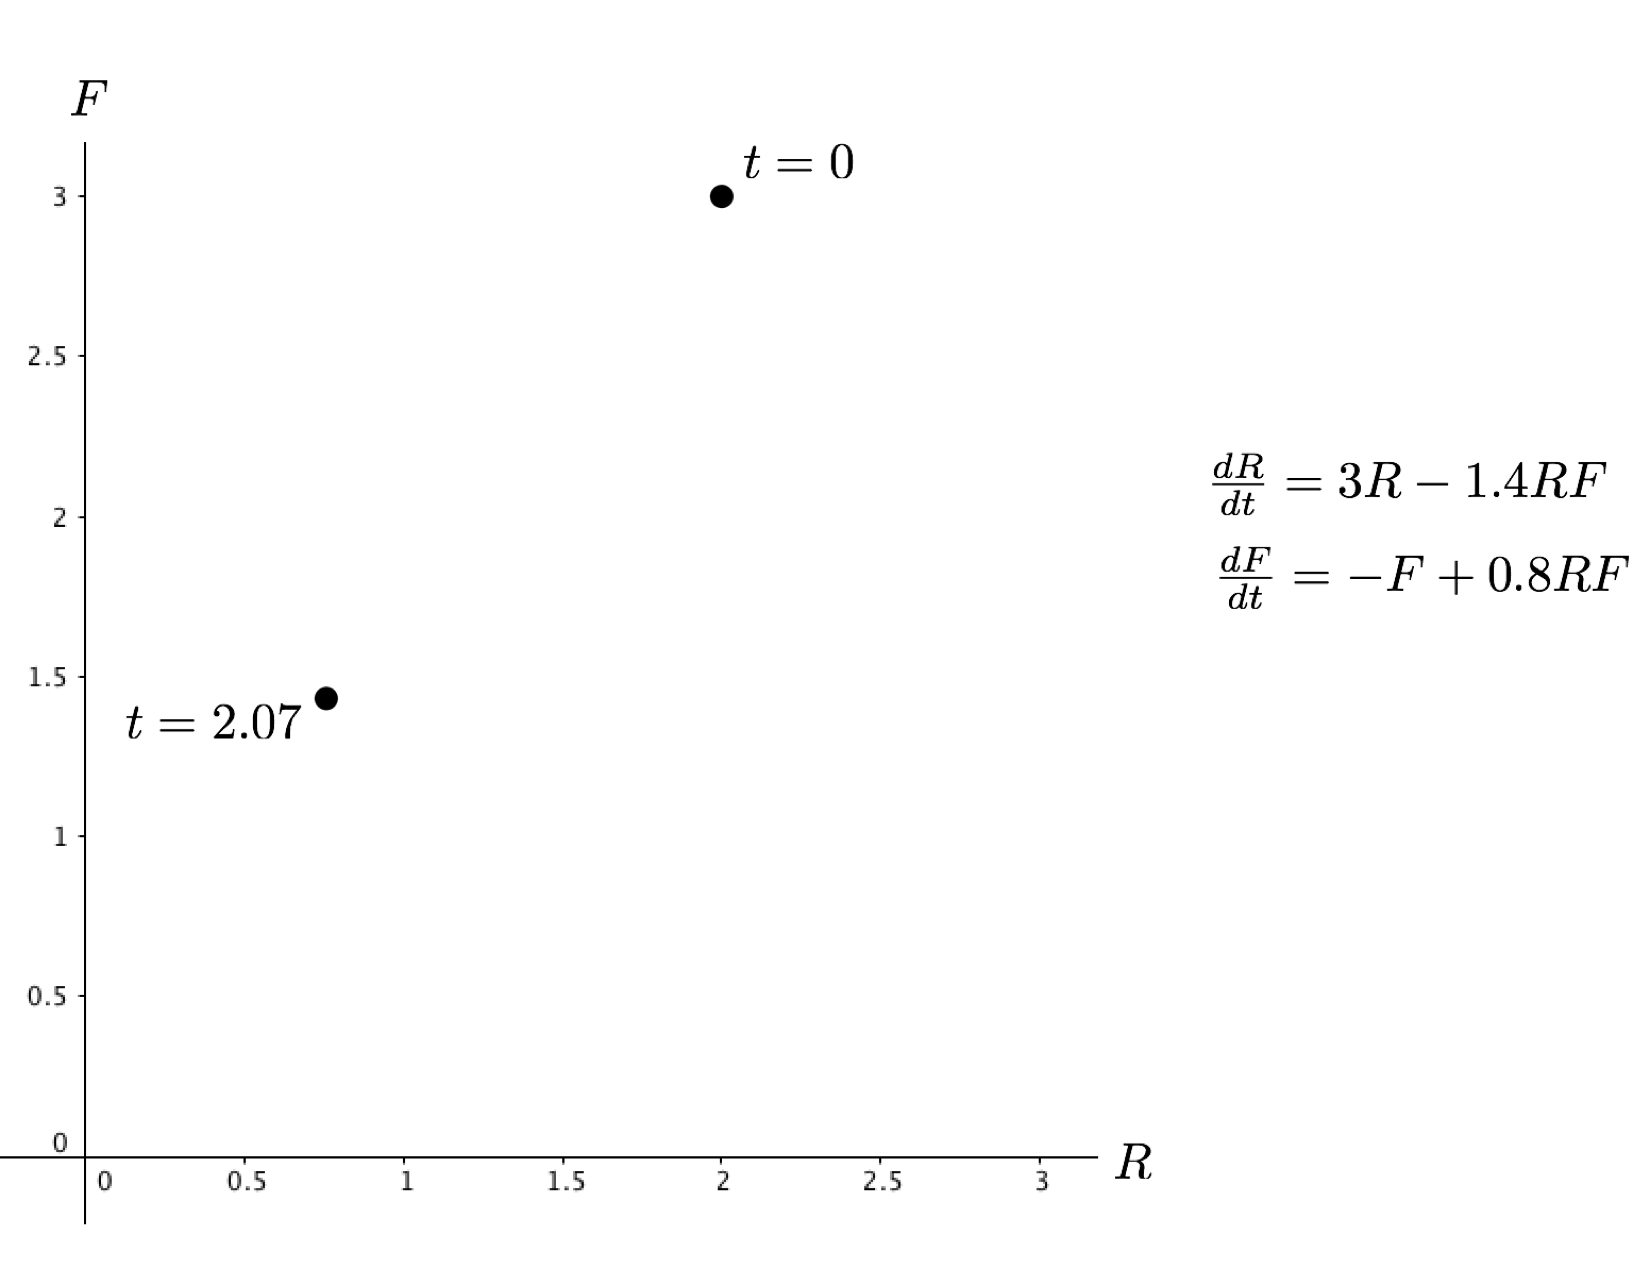
\includegraphics[width=4in]{11/11Clockwise.png}
\end{center}

\item	On the same set of axes from problem \ref{09problem8parta} plot additional vectors at the following points and state what is unique about these vectors. \label{09problem8partb}

\begin{center}
\renewcommand{\arraystretch}{2}
\begin{tabular}{|c|c|c|c|c|}
\hline
$\mathbf{R}$&	$\mathbf{F}$&	$\mathbf{dR/dt}$&	$\mathbf{dF/dt}$&	$\mathbf{dF/dR}$\\\hline
1.25	&0&&&\\\hline			
1.25	&1	&&&\\\hline		
1.25	&2	&&&\\\hline		
1.25	&3	&&&\\\hline	
\end{tabular}

\end{center}
\end{enumerate}
\end{enumerate}
\clearpage

%%%%%%%%%%%%%%%%%%%%%%%%%%
\pagebegin{Vector Fields}

Slope fields are a convenient way to visualize solutions to a single differential equation. For systems of autonomous differential equations the equivalent representation is a \textbf{vector field}. Similar to a slope field, a vector field shows a selection of vectors with the correct slope but with a normalized length. In the previous problem you plotted a few such vectors but typically more vectors are needed to be able to visualize the solution in the phase plane.

\begin{enumerate}[resume]
\item	On a grid where $x$ and $y$ both range from -3 to 3, plot by hand a vector field for the system of differential equations \label{09problem9}
\begin{align*}
	\frac{dx}{dt} &= y-x\\
	\frac{dy}{dt} &= -y\\
\end{align*}
   and sketch in several solution graphs in the phase plane. 
\begin{center}
	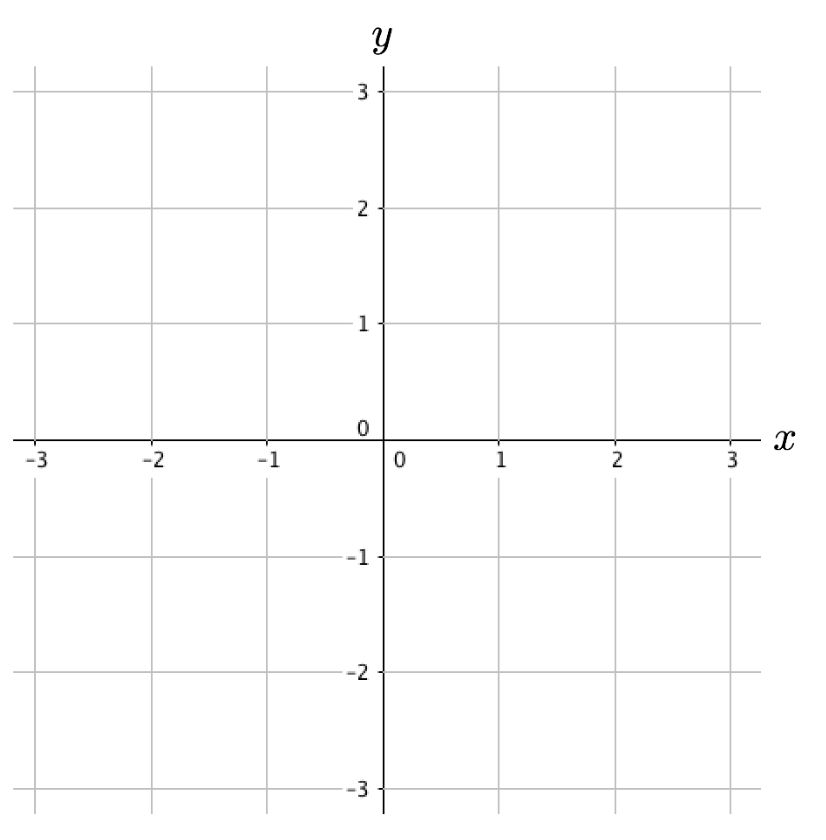
\includegraphics[width=4in]{11/11VectorField1.png}\\
\end{center}
\vfill
 
\item	
\label{09problem10}
\begin{enumerate}
\item You may have noticed in problem \ref{09problem9} that along $x = 0$ all the vectors have the same slope. Similarly for vectors along the $y = x$. Any line or curve along which vectors all have the same slope is called an \textbf{isocline}. An isocline where $dx/dt = 0$ is called an $\mathbf{x}$-\textbf{nullcline} because there is the horizontal component to the vector is zero and hence the vector points straight up or down. An isocline where $dy/dt = 0$ is called a $\mathbf{y}$-\textbf{nullcline} because the vertical component of the vector is zero and hence the vector points left or right. On a grid from -4 to 4 for both axes, plot all nullclines for the following system: \label{09problem10parta}
\begin{align*}
\frac{dx}{dt} &= 3x-1.4xy\\
\frac{dy}{dt} &= -y+0.8xy\\ 
\end{align*}
\begin{center}
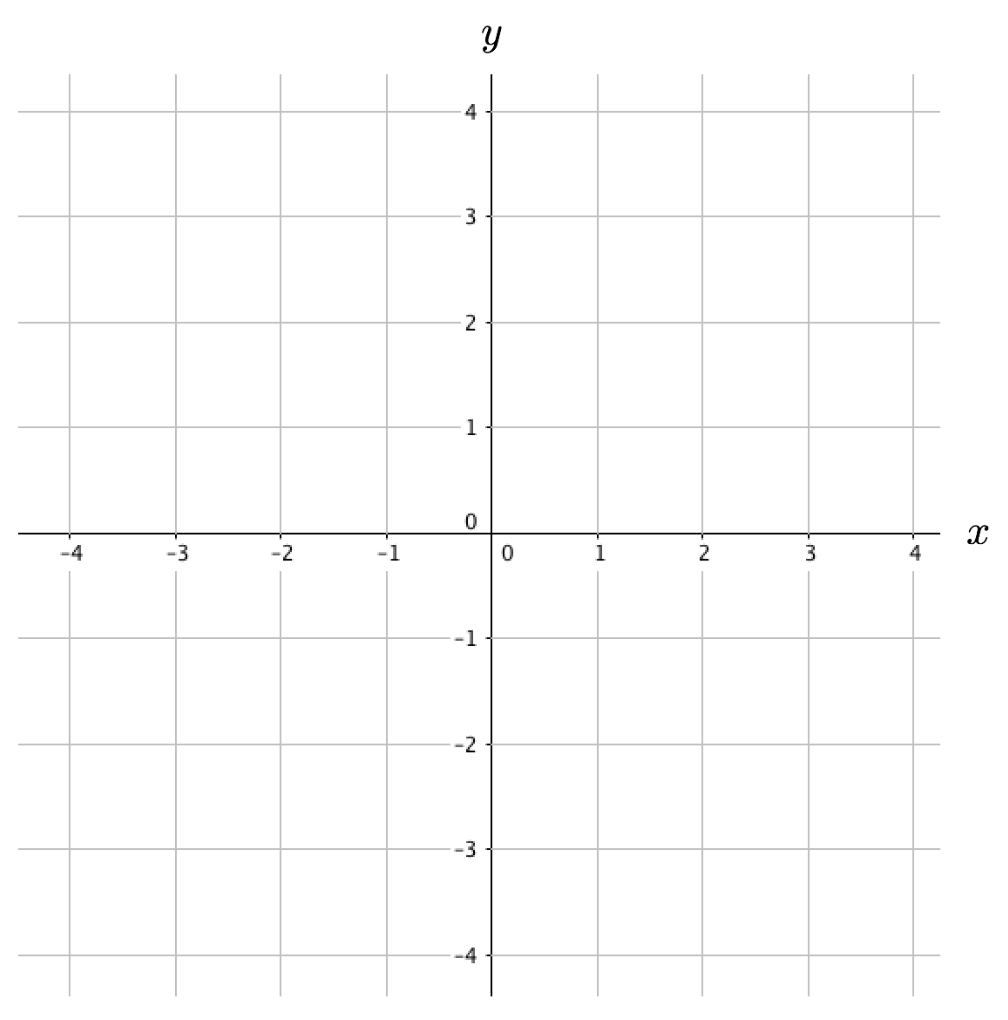
\includegraphics[width=5in]{11/11VectorField2.png}
\end{center}
\item How do these nullclines point to the cyclic nature of the Rabbit-Fox system? \label{09problem10partb}
\end{enumerate}

\clearpage

\item A certain system of differential equations for the variables $R$ and $S$ describes the interaction of rabbits and sheep grazing in the same field.  On the phase plane below, dashed lines show the $R$ and $S$ nullclines along with their corresponding vectors. \label{09problem11}
\begin{enumerate}
\item Identify the $R$ nullclines and explain how you know. \label{09problem11parta}
\item Identify the $S$ nullclines and explain how you know. \label{09problem11partb}
\item Identify all equilibrium points. \label{09problem11partc}
\item Notice that the nullclines carve out 4 different regions of the first quadrant of the $RS$ plane.  In each of these 4 regions, add a prototypical-vector that represents the vectors in that region. That is, if you think the both $R$ and $S$ are increasing in a certain region then, draw a vector pointing up and to the right for that region. \label{09problem11partd}
\item What does this system seem to predict will happen to the rabbits and sheep in this field? \label{09problem11parte}
\begin{center}
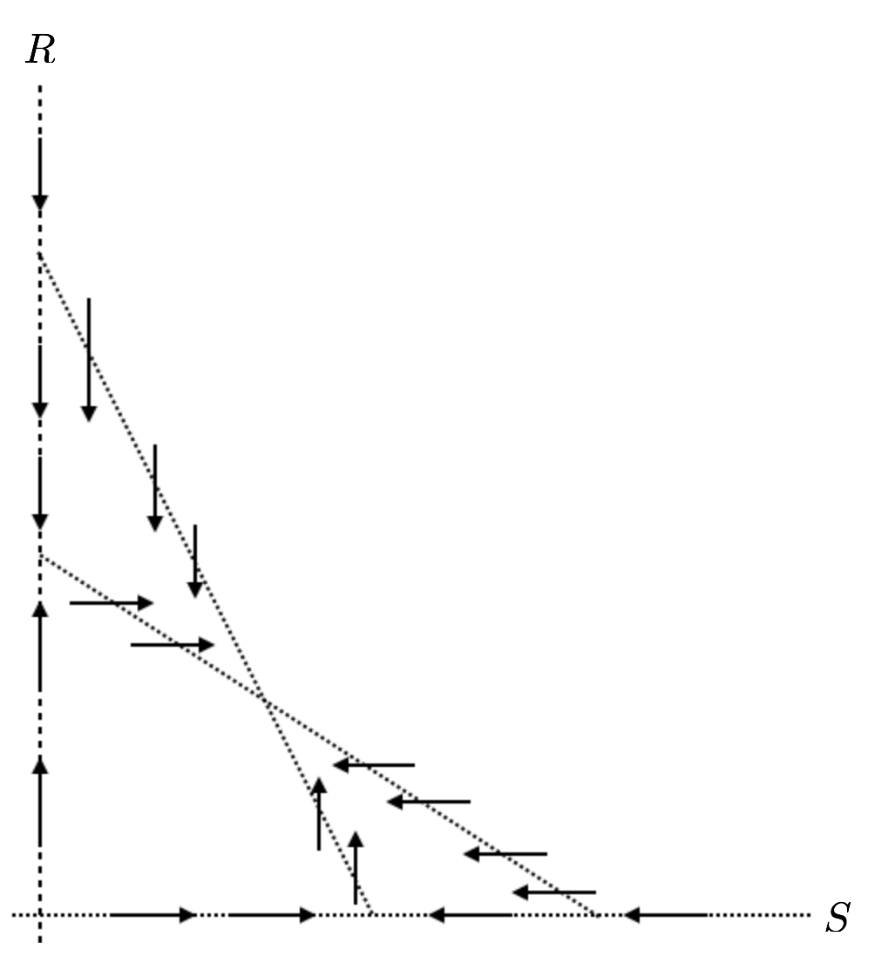
\includegraphics[width=5in]{11/11Nullclines.png}
\end{center}
\end{enumerate}
\end{enumerate}

\clearpage

%%%%%%%%%%%%%%%%%%
%%%%%%%%%%%%%%%%%%%%%%%%%%%%%%%%%%%%%%%%%

Math 3200 \hfill Fundamentals of Differential Equations \hfill Spring 2019

\bigskip

\begin{center}{\large \textbf{Homework \#7, Due Thurs. April 4}} \end{center}
\begin{center}Introduction to the Phase Plane (see Section 5.4 of textbook for further reading)\end{center}

\bigskip

\begin{enumerate}
%\item \label{09HWproblem1}
%\begin{enumerate}
%\item Consider again the crop duster plane problem but this time the red mark slowly drifts toward the center as the propellers rotate as the plane rolls along the runway. Sketch what the four observers see this time. \label{09HWproblem1parta}
%\item	What do the four observers ideally see if the propellers are not rotating and the red mark drifts toward the center at a rate proportional to its distance from the center as the plane rolls along the runway? \label{09HWproblem1partb}
%\end{enumerate}
	
%\item Consider the same system of differential equations from problem \ref{09HWproblem1}. Use the GeoGebra applet \href{https://ggbm.at/U3U6MsyA}{\underline{https://ggbm.at/U3U6MsyA}} to generate predictions for the future number of rabbits and foxes if at time 0 we initially have the following different initial conditions: (i) 200 rabbits and 30 foxes, (ii) 150 rabbits and 40 foxes, and (iii) 400 rabbits and 20 foxes. For each of the different views, graph all three solutions on the same set of axes. \label{09HWproblem2} \\

%\vspace{-0.75in}\hspace{-0.7in}
\includegraphics[width=0.5in]{11/11DEExplorerQR.png}

\item
\begin{enumerate}
\item Referring back to the rabbit and fox system of differential equations ($R$ is hundreds of rabbits and $F$ is tens of foxes), suppose the current number of rabbits is 0 and the number of foxes is $F=2$ (20 foxes). Without using any technology and without making any calculations, what does the system of rate of change equations predict for the future number of rabbits and foxes? Explain your reasoning. \label{09HWproblem3parta}
	\begin{align*}
	\frac{dR}{dt} &= 3R-1.4RF\\
	\frac{dF}{dt} &= -F+0.8RF
\end{align*}

\vspace{-0.75in}\hspace{-0.7in}
\includegraphics[width=0.5in]{11/11DEExplorerQR.png}

\item Use the GeoGebra applet \href{https://ggbm.at/U3U6MsyA}{\underline{https://ggbm.at/U3U6MsyA}} to generate the 3D plot and all three different views or projections of the 3D plot. Show each graph and explain how each illustrates your conclusion in problem \ref{09HWproblem3parta}). \label{09HWproblem3partb}

\item Suppose the current number of rabbits is 0 and the number of foxes is $F=6$ (60 foxes). What does the system of rate of change equations predict for the future number of rabbits and foxes? How and why is this prediction related to the prediction when the initial number of rabbits is 0 and the number of foxes is $F=2$? \label{09HWproblem3partc}
\end{enumerate}

\clearpage

\item Here are three vector fields, A, B, and C. Below the vector fields are some pairs of rate of change equations. Determine which of the pairs match each of the vector fields. Write an explanation of each. \label{09HWproblem4}
\begin{enumerate*}
\item 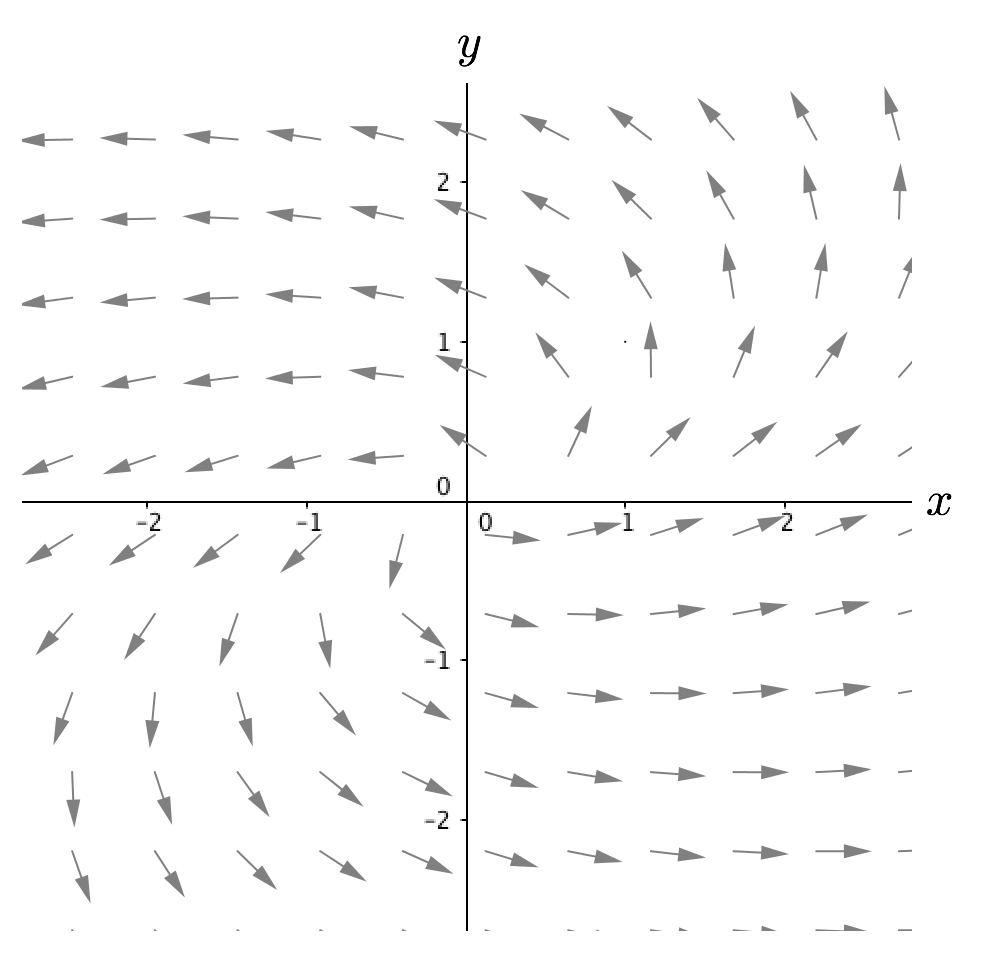
\includegraphics[width=3in]{11/11HWVectorFieldMatchA.png}
\item 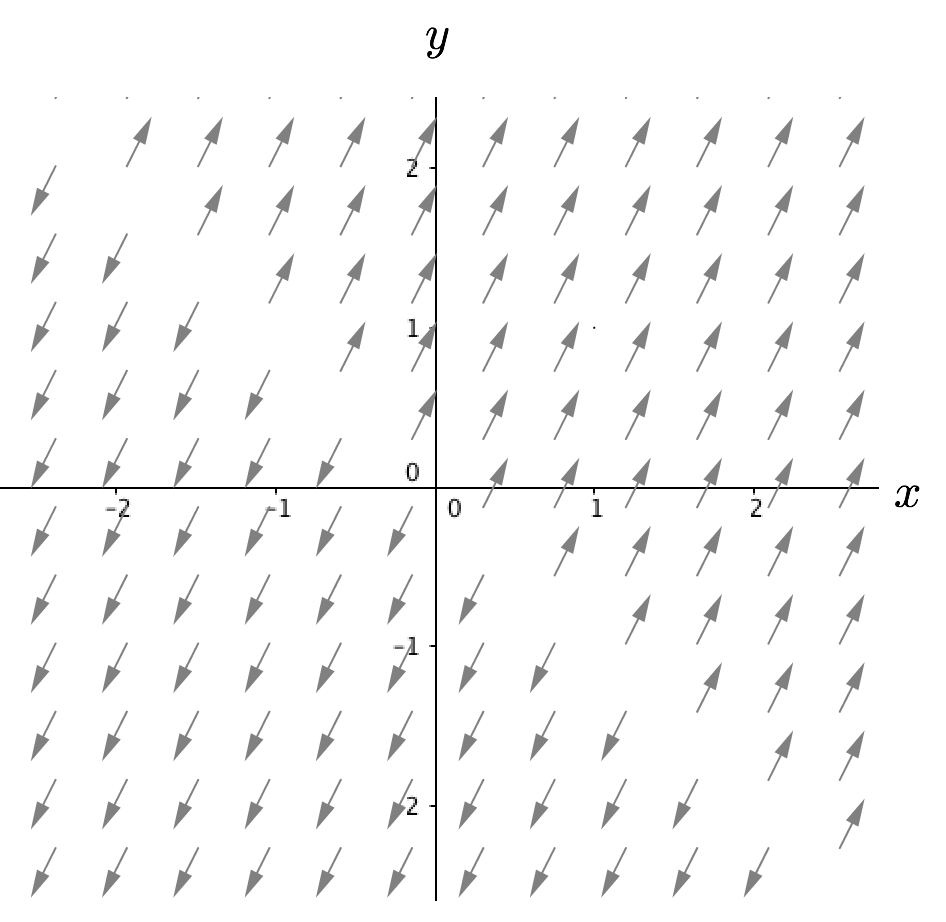
\includegraphics[width=3in]{11/11HWVectorFieldMatchB.png}
\item 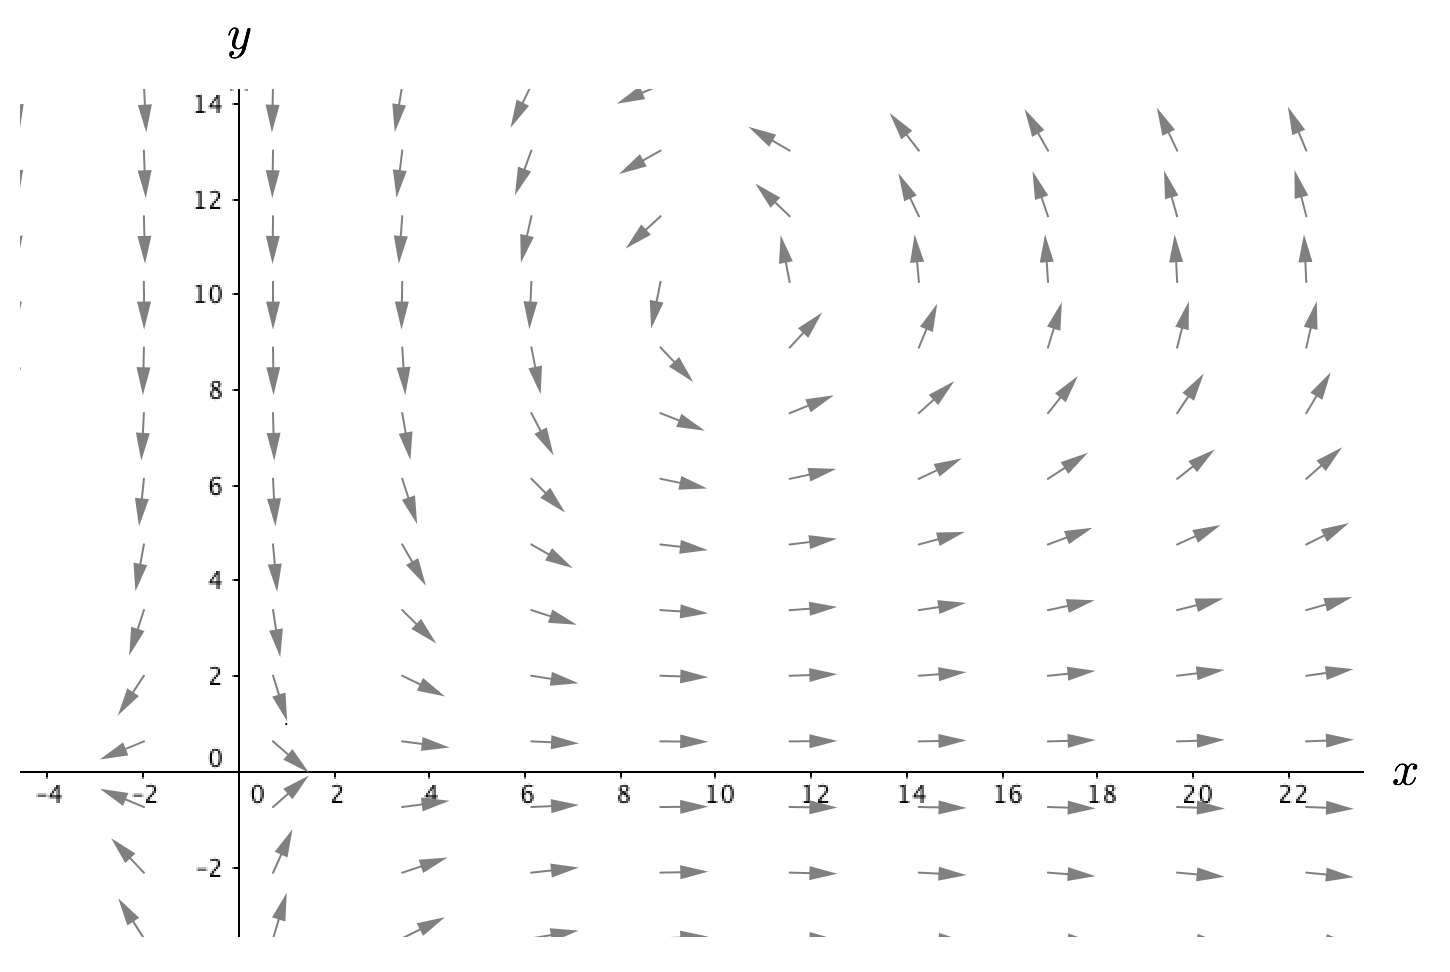
\includegraphics[width=3in]{11/11HWVectorFieldMatchC.png}
\end{enumerate*}
\begin{center}
\begin{enumerate*}
\item[(i)]
$\begin{aligned}
\frac{dx}{dt} &= x+y\\
\frac{dy}{dt} &= -x+y \hspace{.4in}
\end{aligned}$
\item[(ii)]
$\begin{aligned}
\frac{dx}{dt} &= x-0.1xy\\
\frac{dy}{dt} &= -y+0.1xy \hspace{.4in}
\end{aligned}$
\item[(iii)]
$\begin{aligned}
\frac{dx}{dt} &= 2x-3y\\
\frac{dy}{dt} &= x+y \hspace{.4in}
\end{aligned}$
\item[(iv)]
$\begin{aligned}
\frac{dx}{dt} &= x+y\\
\frac{dy}{dt} &= 2x+2y
\end{aligned}$
\end{enumerate*}
\end{center}

\clearpage

\item In previous problems dealing with two species, one of the animals was the predator and the other was the prey. In this problem we study systems of rate of change equations designed to inform us about the future populations for two species that are either competitive (that is both species are harmed by interaction) or cooperative (that is both species benefit from interaction). \label{09HWproblem5}

\begin{enumerate}
\item Which system of rate of change equations describes a situation where the two species compete and which system describes cooperative species? Explain your reasoning. \label{09HWproblem5parta}
\begin{center}
\begin{tabular}{cc}
	 (A)	&	(B)	\\
$\displaystyle \begin{aligned} \frac{dx}{dt} &= -5x+2xy\\ \frac{dy}{dt} &= -4y+3xy \end{aligned}$ &$\displaystyle \begin{aligned} \frac{dx}{dt} &= 3x(1-\frac{x}{3})-\frac{1}{10}xy\\ \frac{dy}{dt} &= 2y(1-\frac{y}{10})-\frac{1}{5}xy \end{aligned}$ 
\end{tabular}
\end{center}

\item	For system (A), plot all nullclines and use this plot to determine all equilibrium solutions. Verify your equilibrium solutions algebraically. \label{09HWproblem5partb}
\item	Use your results from \ref{09HWproblem5partb} to sketch in the long-term behavior of solutions with initial conditions anywhere in the first quadrant of the phase plane. For example, describe the long-term behavior of solutions if the initial condition is in such and such region of the first quadrant. Provide a sketch of your analysis in the $x$-$y$ plane and write a paragraph summarizing your conclusions and any conjectures that you have about the long-term outcome for the two populations depending on the initial conditions. \label{09HWproblem5partc} 

\end{enumerate}
\item Consider the following systems of rate of change equations:

\begin{center}
	\begin{tabular}{cc}
	\underline{\textbf{System A}}	&					\underline{\textbf{System B}}\\
$\displaystyle \begin{aligned} \frac{dx}{dt} &= 3x(1-\frac{x}{10})-\frac{1}{20}xy\\ \frac{dy}{dt} &=-5y+\frac{xy}{20} \end{aligned}$  	&			$\displaystyle \begin{aligned} \frac{dx}{dt} &= 3x-\frac{xy}{100}\\ \frac{dy}{dt} &=15y(1-\frac{y}{17})+25xy \end{aligned}$ 
	\end{tabular}
\end{center}

In both of these systems, $x$ and $y$ refer to the number of two different species at time $t$. In particular, in one of these systems the prey are large animals and the predators are small animals, such as piranhas and humans. Thus it takes many predators to eat one prey, but each prey eaten is a tremendous benefit for the predator population. The other system has very large predators and very small prey. \label{09HWproblem6}

\begin{enumerate}
\item For both systems of differential equations, what does $x$ represent? The predator or the prey? Explain. \label{09HWproblem6parta}
\item	What system represents predator and prey that are relatively the same size? Explain. \label{09HWproblem6partb}
\item	For system (A), plot all nullclines and use this plot to determine all equilibrium solutions. Verify your equilibrium solutions algebraically.\label{09HWproblem6partc}
\item	Use your results from \ref{09HWproblem6partc} to sketch in the long-term behavior of solutions with initial conditions anywhere in the first quadrant of the phase plane. For example, describe the long-term behavior of solutions if the initial condition is in such and such region of the first quadrant. Provide a sketch of your analysis in the $x$-$y$ plane and write a paragraph summarizing your conclusions and any conjectures that you have about the long-term outcome for the two populations depending on the initial conditions. \label{09HWproblem6partd}
\end{enumerate}

\clearpage

\item Provide sketches of $x$ vs $t$ and $y$ vs $t$ for each of the following phase planes and solution curves. \label{09HWproblem7}
\begin{enumerate*}
\item 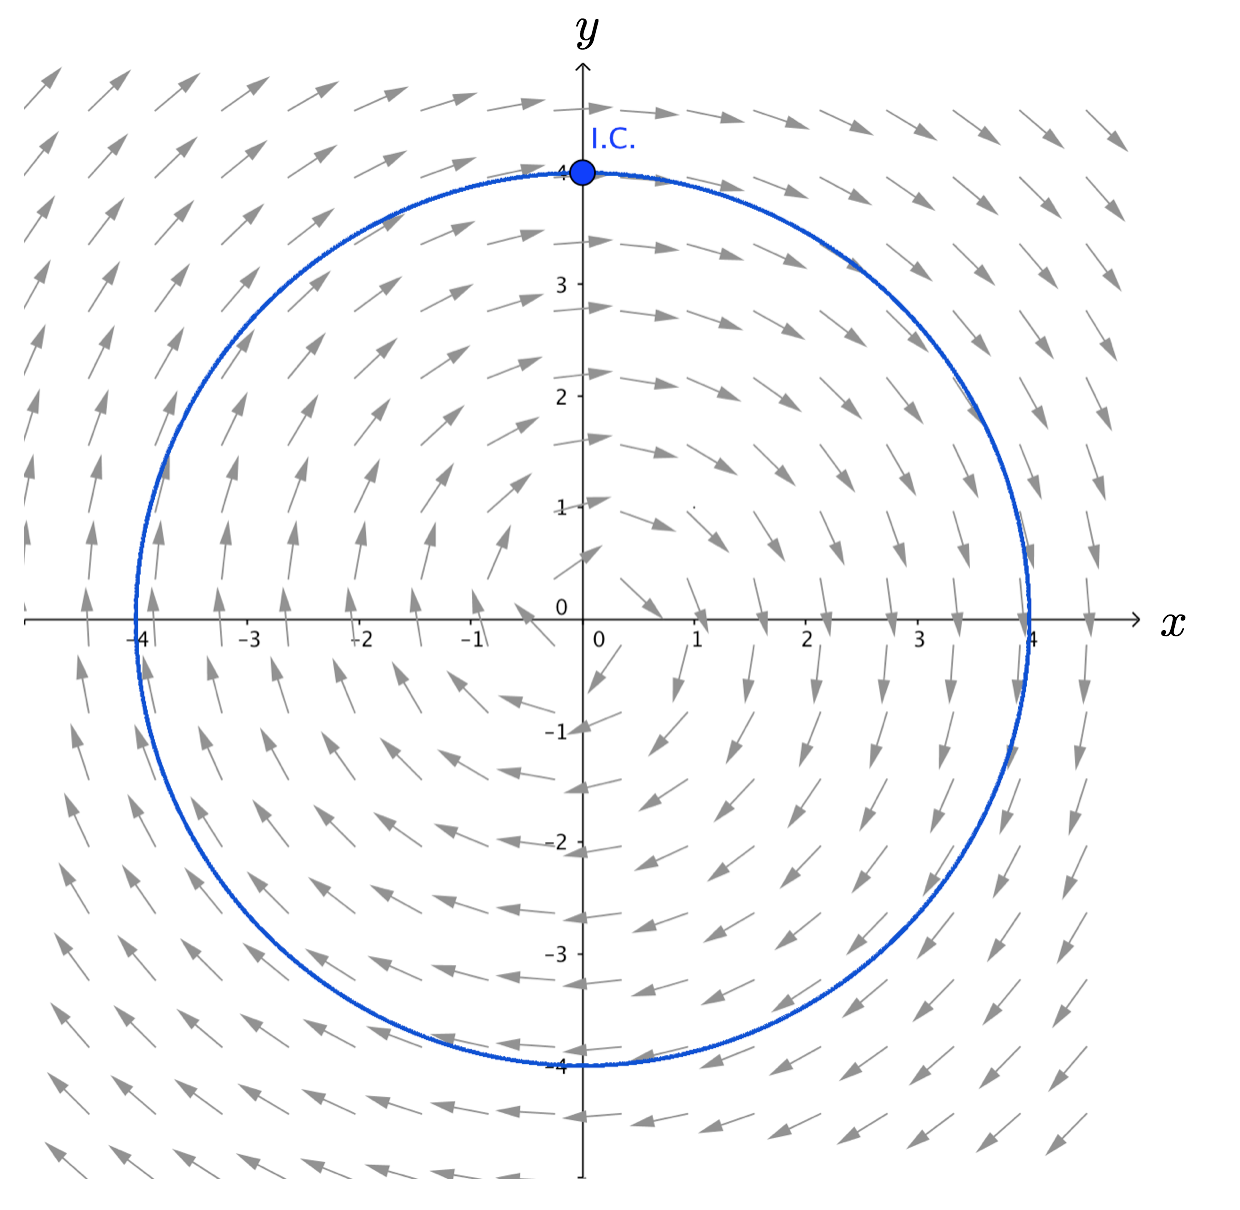
\includegraphics[width=3in]{11/11HWPhasePlaneSolution1.png} \label{09HWproblem7parta}
\item 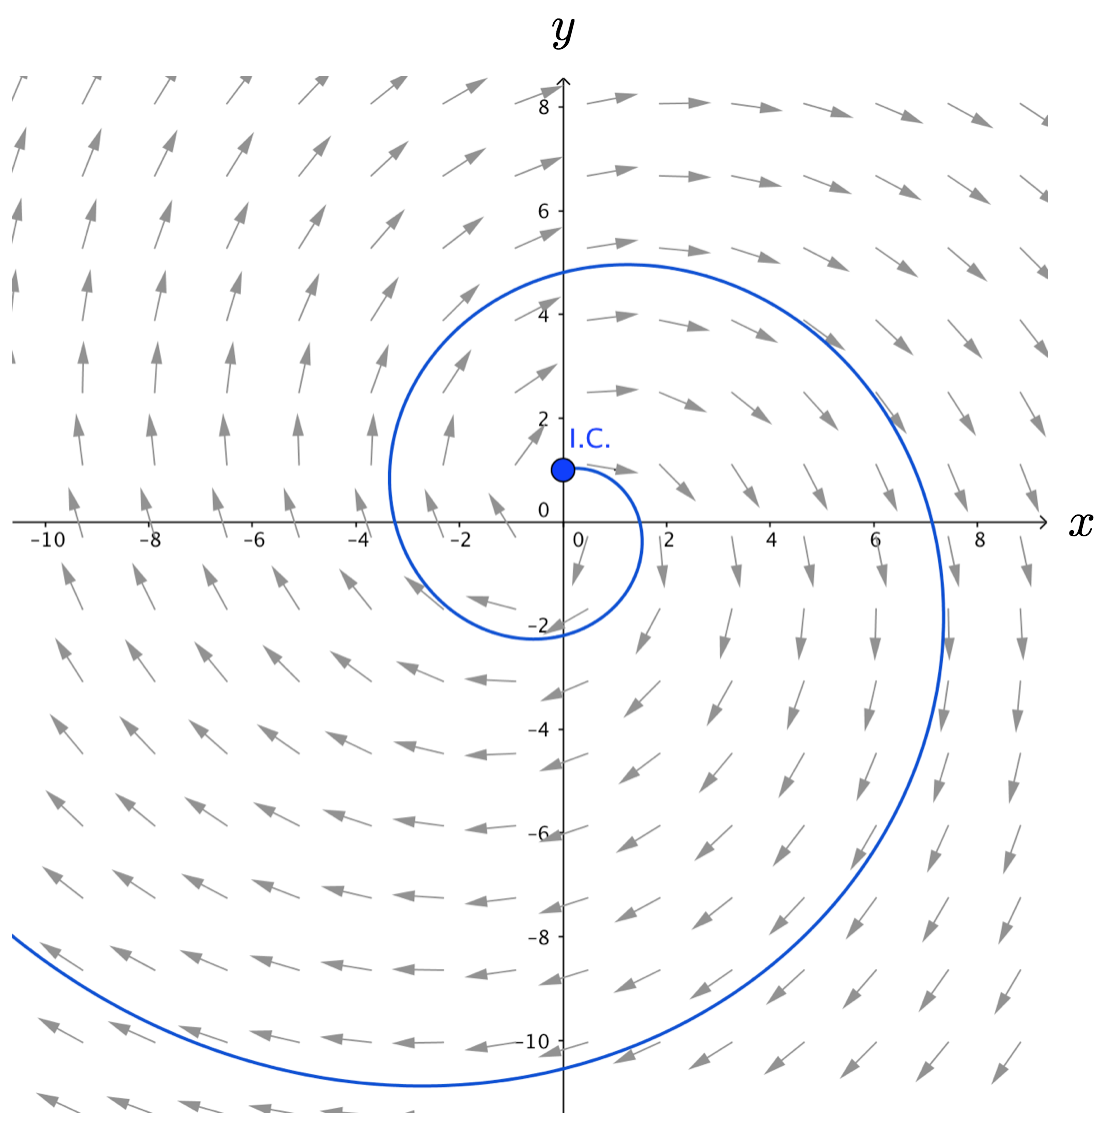
\includegraphics[width=3in]{11/11HWPhasePlaneSolution2.png} \label{09HWproblem7partb}
\item 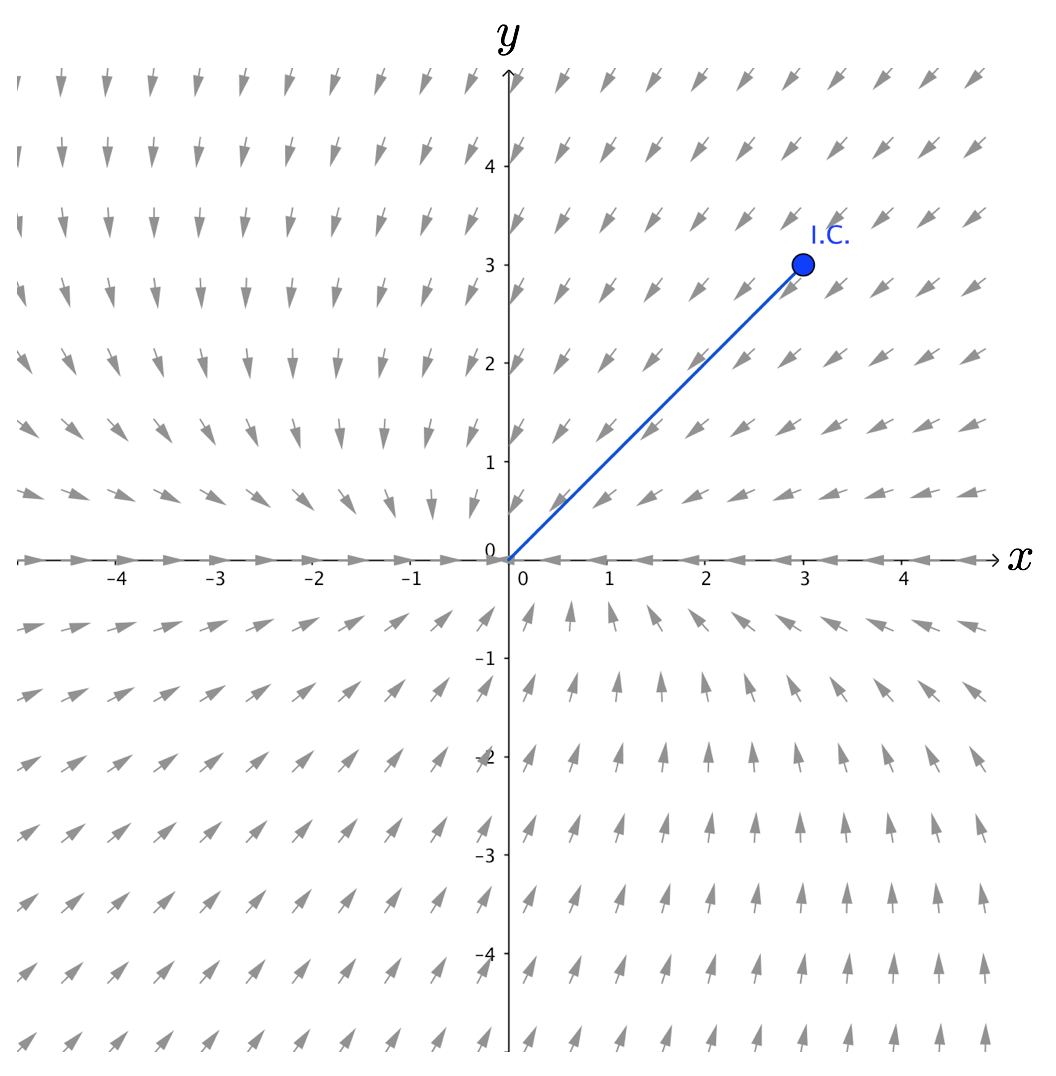
\includegraphics[width=3in]{11/11HWPhasePlaneSolution3.png} \label{09HWproblem7partc}
\item 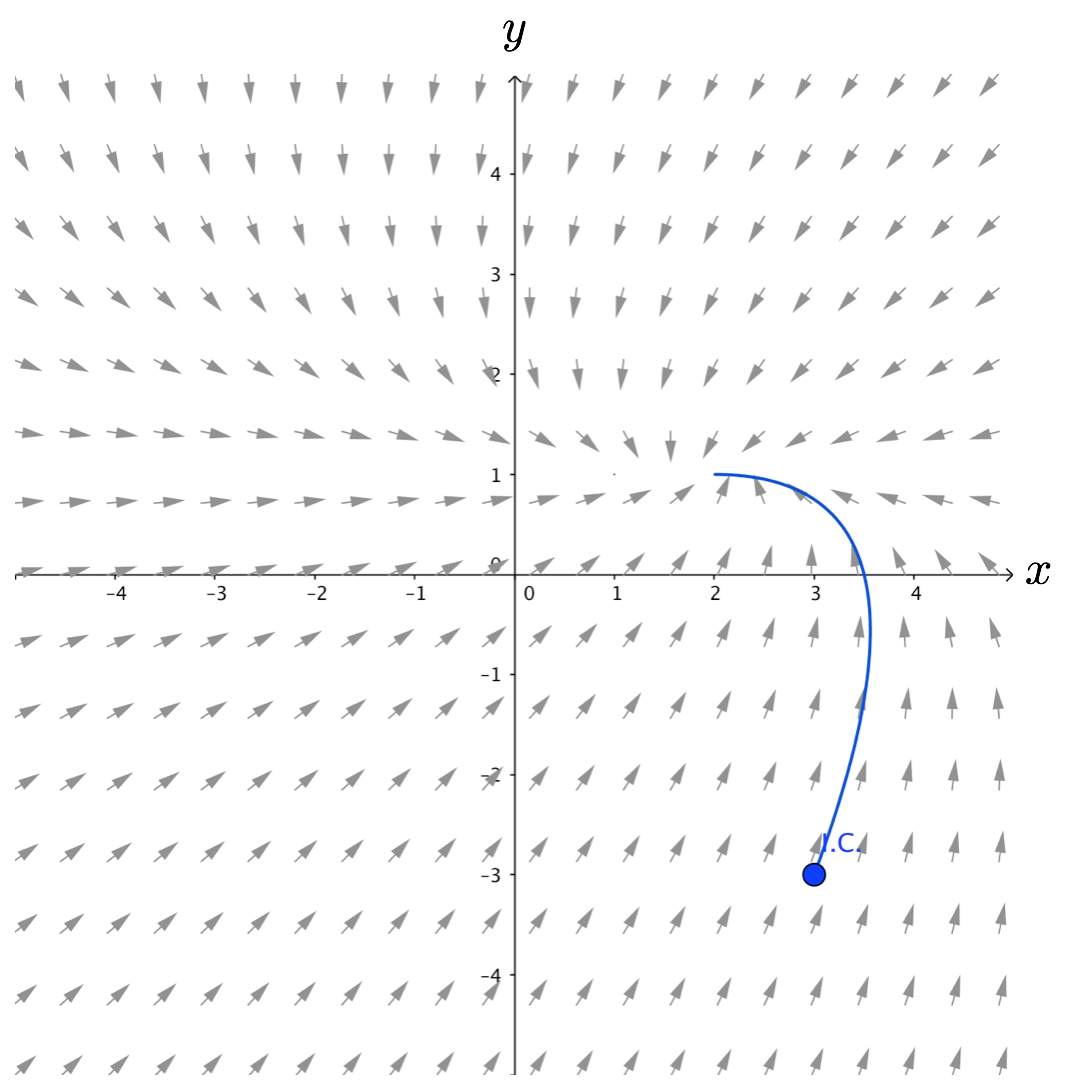
\includegraphics[width=3in]{11/11HWPhasePlaneSolution4.png} \label{09HWproblem7partd}
\end{enumerate*}
\end{enumerate}
